
\documentclass[a4paper,10pt]{article}
\usepackage[utf8]{inputenc} %Codificacion utf-8
\usepackage{graphicx}
\usepackage{enumerate}
\usepackage{fancyhdr}
\usepackage{hyperref}
\usepackage{multirow} % Required for multirows
\usepackage[spanish, activeacute]{babel} %Definir idioma español
% \usepackage[margin=3cm]{geometry}
\hypersetup{
    colorlinks=true,
    linkcolor=black,
    filecolor=magenta,
    urlcolor=cyan,
}
\pagestyle{fancy}

\lhead{Análisis clínicos III}
\rfoot{Página \thepage}
\lfoot{Diego Rodríguez Riera}
\cfoot{Bases de Datos}
\newcommand\tab[1][1cm]{\hspace*{#1}}

\title{Análisis clínicos III\\{\small rev 2}}
\author{Diego Rodríguez Riera}
\date{\today}

\begin{document}

\maketitle
\pagebreak
\tableofcontents
\pagebreak

\section{Definición del problema.}
\paragraph{}
A lo largo de las clases impartidas el alumnado ha comprendido la importancia de una descripción rigurosa del problema del mundo real con el fin de poder construir un modelo conceptual del mismo que sirva de base para la representación lógica del problema y su tratamiento mediante la tecnología de bases de datos.
\paragraph{}
Por lo tanto, como paso previo al uso de un modelo de datos para la construcción del modelo conceptual, es necesario llevar a cabo el estudio exhaustivo del problema planteado (Gestión de Análisis Clínicos).
\paragraph{}
En este estudio se describirán todos los elementos de información que participan en el problema, su definición, descripción y medida, así como las relaciones existentes entre los elementos de información.
\paragraph{}
Además, se consideraran las restricciones innatas al problema existentes en los elementos de información y las relaciones que existen entre los mismos.
\paragraph{}
Dado que aún no han sido impartidos los conceptos sobre el modelo conceptual Entidad-Interrelación, en esta actividad no se utilizará este modelo para la descripción del problema. Se trata que el alumnado estudie, comprenda y describa el problema, y los elementos de información que deben considerarse y sus características teniendo en cuenta los procesos que deberán considerarse para la gestión de esta información.
\pagebreak

\section{Análisis del problema.}
\paragraph{}
El problema esta planteado en el dominio de los análisis clínicos con metodos actuales, estos se centran en varios factores los cuales varían según la edad, sexo y enfermedades del cliente.
\paragraph{}
Estos factores supondrán en gran parte la complejidad de la base de datos, especificamente el dominio de los datos de la base de datos en los cuales tendrán que estar representadas en estas restricciones.
\section{Factores a tener en cuenta.}
\label{section:factoresatenerencuenta}
\paragraph{}
Los factores que más influyen en un análisis clínico son los siguientes:
\begin{itemize}
	\item Edad.
	\item Sexo.
	\item Embarazo.
	\item Enfermedades.
	\item Consumo de cafeína, tabaco o alcohol.
	\item Situaciones de estrés o ansiedad.
	\item Ejercicio Físico antes de la realización de la prueba.
\end{itemize}

\section{Mediciones recogidas por los análisis.}
Un ejemplo de las medidas obtenidas podría ser el siguiente:
\subsection{Analisis de sangre.}
Glucosa, Colesterol total, Colesterol HDL, Colesterol LDL, Triglicéridos, Ácido úrico, Transaminasas, GOT/ASAT, GPT/ALT, Proteínas totales, Albúmina, Bilirrubina total, Hematíes (eritrocitos), Hemoglobina, Hematocrito, V.C.M., H.C.M., C.H.C.M., Leucocitos, Neutrófilos, Linfocitos, Monocitos, Eosinófilos, Basófilos, Hierro, Ferritina, Plaquetas, V.S.G., Fibrinógeno \subsection{Analisis de saliva.}
pH, Sodio, Potasio, cloro
\subsection{Analisis de orina.}
Albúmina, Densidad, pH, Glucosa, Proteínas, Cetonas, Urobilinógeno y bilirrubina, Nitrito, Cristales, Células epiteliales, cilindros, Cuerpos cetónicos, Osmolalidad, Glóbulos rojos, Glóbulos blancos, Cetona, Creatinina
\pagebreak

\section{Diagrama de clases de análisis.}
\paragraph{}
Para poder implementar todas las restricciones de dominio, tendremos que crear el siguiente árbol de generalización para los analisis:\\
% \vspace{0.7cm}\\
\begin{figure}[hbt]
	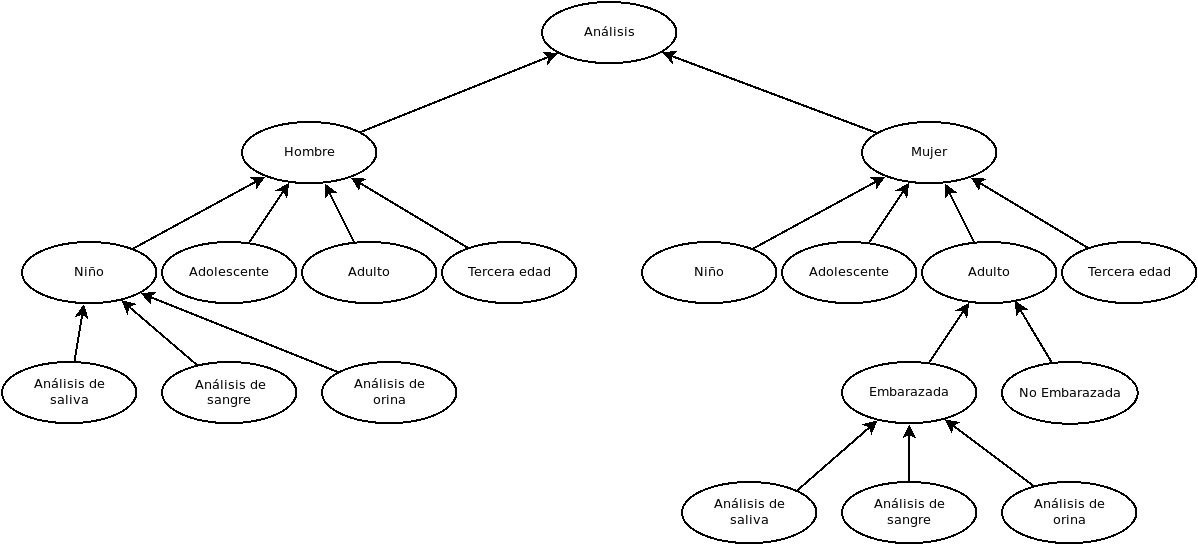
\includegraphics[width=\textwidth]{img/analisis.png}
	\caption{Diagrama de clases de análisis.}
	\label{fig:diagramaanalisis}
\end{figure}
\paragraph{}
Para poder representar todas las restricciones de dominio que presentan los analisis, tendremos que efectuar restricciones de dominio de la información tanto en sexo, edad, tipo de análisis y finalmente validez del análisis.
\paragraph{}
A esto le tenemos que añadir, en el caso de la mujer el posible estado de embarazada a partir de la adolescencia.
\subsection{Atributos de los análisis}
\paragraph{}
Cada análisis estara compuesto por diversos atributos los cuales haran referencia tanto a los valores de las mediciones obtenidas en el análisis del pariente, como a los umbrales de normalidad de dichas mediciones.
\paragraph{}
El analista debera de tener acceso a una serie de factores modificadores de los resultados del análisis como los citados anteriormente en la sección \ref{section:factoresatenerencuenta}, \nameref{section:factoresatenerencuenta}, estos seran almacenados como observaciones para su posterior uso por parte del personal cualificado.

\pagebreak
\subsection{Restricciones de dominio de la información.}
\subsubsection{Restricciones de dominio segun el sexo.}
\paragraph{}
Podemos diferenciar entre sexos ya que los umbrales de normalidad en los análisis pueden ser distintos en cada sexo.

\subsubsection{Restricciones de dominio segun la edad.}
\paragraph{}
Debido a los diferentes máximos y mínimos entre las distintas franjas de edades, haremos una distinción entre diferentes grupos de edades diferentes, una posible clasificación podria ser la siguiente:
\begin{table}[hbt]
		\begin{center}
		\begin{tabular}{|c|c|}\hline
			subclase & franja de edad \\ \hline
			Niño & $<$10 \\ \hline
			Adolescente & 10-25 \\ \hline
			Adulto & 25-70 \\ \hline
			Tercera edad & $>$70 \\ \hline
		\end{tabular}
		\caption{Restricciones de dominio segun la edad}
	\end{center}
\end{table}
\subsubsection{Restricciones de dominio segun la naturaleza del análisis}
\paragraph{}
Segun la naturaleza del análisis podemos distinguir entre varios tipos, en este ejemplo se consideran tres tipos de analiticas:
\begin{itemize}
	\item Análisis de sangre
	\item Análisis de saliva
	\item Análisis de orina
\end{itemize}
\subsubsection{Restricciones de dominio segun el embarazo.}
\paragraph{}
En el caso de la mujer, habrá un nivel extra de especialización, uno para el estado no embarazada y otro para el estado embarazada, la entidad análisis se especificará en uno u otro dependiendo del estado de la mujer en el momento del análisis, ya que este afectara en gran medida a muchos umbrales de normalidad.
\pagebreak
\subsection{Consideraciones segun la normalidad del análisis}
\paragraph{}
En lo que respecta la normalidad del análisis, estos podran ser clasificados como $"$normales$"$ o $"$anormales$"$.
\paragraph{}
Los análisis normales son todos aquellos cuyas mediciones se encuantran en el umbral de aceptación de la subclase a la que isntancian, si esto es cierto para todas las mediciones de susodicho análisis, el analisis sera considerado como normal.
\paragraph{}
En el caso de que una o varias mediciones se salgan del umbral de aceptación de dicha subclase, este será clasificado como $"$Análisis Anormal$"$.
\paragraph{}
Los umbrales seran definidos por un especialista en la materia devido a su alta complejidad.
\paragraph{}
Si el análisis es clasificado como anormal, este será marcado como tal en un sitio visible del impreso.
\paragraph{}
A demas, antes de la impresión, se evaluara si la medición esta entre los parametros máximos y mínimos, si esta no lo esta la medición se marcará en otro color al del texto normal.
\paragraph{}
Nótese que solo el sexo, edad, y en el caso de la mujer, si esta está embarazada se han tenido en cuneta para los máximos y los mínimos, el resto de factores se almacenaran en la variable $"$observaciones$"$ en las intancias de las sublases correspondientes al tipo de análisis, para su posterior consideración por el personal cualificado.
\pagebreak

\section{Diagrama de clases de personas.}
\paragraph{}
Hay tres tipos de personas, el paciente al que se realiza el análisis, el Doctor que receta el análisis el analista que lleva a cabo el análisis en el laboratorio.
\paragraph{}
El diagrama de abstracción seria el siguiente:
\vspace{0.5cm}
\begin{center}
	\begin{figure}[hbt]
		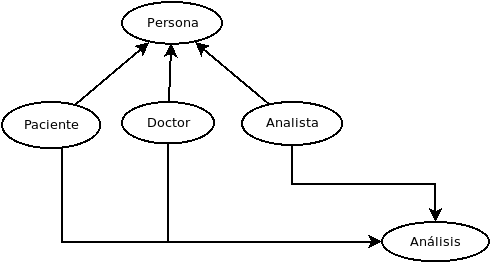
\includegraphics[width=\textwidth]{img/personas.png}
		\caption{Diagrama de clases de personas.}
		\label{fig:diagramapersonas}
	\end{figure}
\end{center}
\paragraph{}
Para que un análisis sea realizado este debe de ser mandado por un médico a excepción de casos particulares.
\paragraph{}
Las atributos que se guardarán de las distintas clases serán las siguientes:
\begin{itemize}
	\item {\bf Paciente}: \underline{numero de la seguridad social}, sexo, fecha de nacimiento y lugar de nacimiento.
	\item {\bf Doctor}: \underline{dni}, fecha de nacimiento y campo o especialidad.
	\item {\bf Analista}: \underline{dni}, fecha de nacimiento, campo o especialidad y especialidad como analista.
\end{itemize}
\paragraph{}
Tanto los médicos como los analistas tendrán estar titulados con las titulaciones correspondientes a la tarea desempeñada.
\paragraph{}
Las claves principales estan marcadas con subrayado en los atributos de las clases Paciente, Doctor Y Analista
\paragraph{}
Cada análisis tiene un id único, este es generado automáticamente y es incremental, además, el análisis guarda de quien es el análisis (paciente), quien lo ha realizado (analista) y quien lo ha encargado (el doctor).
\paragraph{}
Referenciando a la figura ~\ref{fig:diagramaanalisis}, y figura ~\ref{fig:diagramapersonas} la multiplicidad de la relacción entre analisis y las diferentes especializaciones de la entidad persona, son las siguientes:
\paragraph{Paciente-Análisis}
Devido a que un paciente podra efectuar multiples análisis, la relacción sera de 1:N, ya que un análisis será solo de un cliente.
\paragraph{Doctor-Análisis}
De igual manera que la relación Paciente-Análisis, esta re-
lacción tiene la multiplicidad 1:N, ya que un análisis solo puede como máximo
ser recetado por un doctor, pero en ciertos escenarios, no hace falta un doctor
que lo recete.

\paragraph{Analista-Análisis}
 Con multiplicidad N:N, ya que un análisis puede ser lle-
vado a cabo por varios analistas.

\section{Máquinas.}
En el laboratorio existen tres tipos de maquinas que pueden escribir o leer de un análisis, estas están representadas en el siguiente diagrama:
% \vspace{0.5cm}\\
% 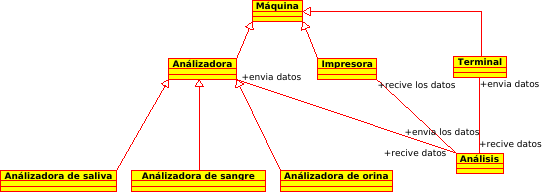
\includegraphics[width=\textwidth]{img/maquinas.png}
\paragraph{}
Como se puede observar, de la entidad maquina, se especializan tres clases:
\begin{itemize}
	\item {\bf Análizadora} Maquina encargada de obtener automáticamente los análisis de las muestras del paciente, a su vez, esta se especializa en tres subclases, una por cada tipo de análisis:
	\begin{itemize}
		\item {\it Análizadora de sangre}.
		\item {\it Análizadora de saliva}.
		\item {\it Análizadora de orina}.
	\end{itemize}
	Estas maquinas pueden obtener ciertos resultados por ellas mismas sin intervención humana mas allá del posicionamiento de las muestras.
	\item {\bf Impresora}: Encargada de imprimir todo documento que se le mande.
	\item {\bf Terminal}: Debido a que no todas las mediciones podrán hacerse automáticamente por las máquinas, algunas muestras tendrán que ser analizadas por los analistas, estos entonces podrán introducir los resultados a travez de una terminal en el laboratorio.
\end{itemize}
\paragraph{}
Una vez completado el análisis, se mandara un documento generado a partir de los datos del análisis al servidor de impresión para su posterior recogida por el doctor que la encargo.\\

% \pagebreak
% \section{Vista general.}
% \paragraph{}
% Gran parte del diagrama de análisis ha sido omitido.\\
% \vspace{0.7cm}\\
% 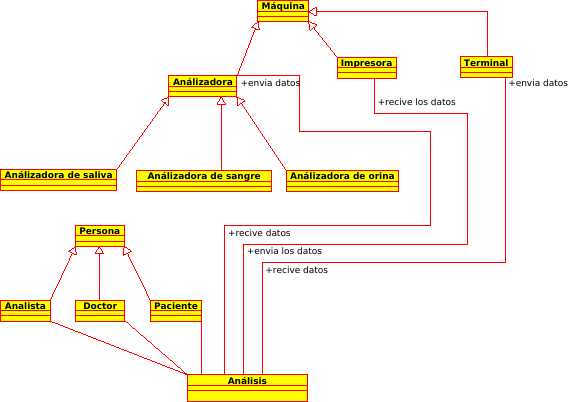
\includegraphics[width=\textwidth]{img/all.png}




%%%%%%%%%%%%%%%%%%%%%%%%%%%%%%%%%%%%%%%%%%%%%%%%%%%%%%%%%%%%%%%%%%%%%%%%%%%%%%%%
%%%%%%%%%%%%%%%%%%%%%%%%%%%%%%%%%%%%%%%%%%%%%%%%%%%%%%%%%%%%%%%%%%%%%%%%%%%%%%%%
%                           commented out things
%%%%%%%%%%%%%%%%%%%%%%%%%%%%%%%%%%%%%%%%%%%%%%%%%%%%%%%%%%%%%%%%%%%%%%%%%%%%%%%%
%%%%%%%%%%%%%%%%%%%%%%%%%%%%%%%%%%%%%%%%%%%%%%%%%%%%%%%%%%%%%%%%%%%%%%%%%%%%%%%%




% \section{Tabla de valores aceptables}
% \subsection{Análisis de sangre}
% \begin{center}
% 	\begin{tabular}{|c|c|c|c|c|c|c|c|c|c|} \hline
%
% 		% header
%
% 		\multirow{2}{*}{medida} & \multicolumn{4}{|c|}{Hombre} & \multicolumn{4}{|c|}{Mujer} & \multirow{2}{*}{unidades} \\ \cline{2-9}
% 		& 0-10 & 10-20 & 20-50 & 50+ & 0-10 & 10-20 & 20-50 & 50+ & \\ \hline
%
% 		% data
%
% %Glucosa,
%
% Glucosa & 100-180 & \multicolumn{3}{|c|}{90-130} & 100-180 &  \multicolumn{3}{|c|}{90-130} & mg/dL \\ \hline
% Colesterol total & \multicolumn{2}{c|}{$<$170} & \multicolumn{2}{c|}{125-200} &\multicolumn{2}{c|}{$<$170} & \multicolumn{2}{c|}{125-200} & mg/dL\\ \hline
% Colesterol HDL  &\multicolumn{4}{c|}{$<$100} &\multicolumn{4}{c|}{$<$100} & mg/dL\\ \hline
% Triglicéridos &  &  &  &  &  &  & & & \\ \hline
% Ácido úrico &  &  &  &  &  &  & & & \\ \hline
% Transaminasas &  &  &  &  &  &  & & & \\ \hline
% GOT/ASAT &  &  &  &  &  &  & & & \\ \hline
% GPT/ALT &  &  &  &  &  &  & & & \\ \hline
% Proteínas totales &  &  &  &  &  &  & & & \\ \hline
% Albúmina &  &  &  &  &  &  & & & \\ \hline
% Bilirrubina total &  &  &  &  &  &  & & & \\ \hline
% Hematíes (eritrocitos) &  &  &  &  &  &  & & & \\ \hline
% Hemoglobina &  &  &  &  &  &  & & & \\ \hline
% Hematocrito &  &  &  &  &  &  & & & \\ \hline
% V.C.M. &  &  &  &  &  &  & & & \\ \hline
% H.C.M. &  &  &  &  &  &  & & & \\ \hline
% C.H.C.M. &  &  &  &  &  &  & & & \\ \hline
% Leucocitos &  &  &  &  &  &  & & & \\ \hline
% Neutrófilos &  &  &  &  &  &  & & & \\ \hline
% Linfocitos &  &  &  &  &  &  & & & \\ \hline
% Monocitos &  &  &  &  &  &  & & & \\ \hline
% Eosinófilos &  &  &  &  &  &  & & & \\ \hline
% Basófilos &  &  &  &  &  &  & & & \\ \hline
% Hierro &  &  &  &  &  &  & & & \\ \hline
% Ferritina &  &  &  &  &  &  & & & \\ \hline
% Plaquetas &  &  &  &  &  &  & & & \\ \hline
% V.S.G. &  &  &  &  &  &  & & & \\ \hline
% Fibrinógeno &  &  &  &  &  &  & & & \\ \hline
%
%
% 	\end{tabular}
% \end{center}


% \raggedleft Document written in \LaTeX{}
\end{document}
